\chapter{Test Cases}\label{chap:test}

This thesis carries out tests for \acf{OBW} measurement, \acf{PSD} measurement, and \acf{RxBlocking} measurement. The definition, limits and the procedure for each test case are mentioned in the subtopics below.

\section{\acl{OBW} measurement}
\label{sec:obw}

The \acf{OBW} is the bandwidth that contains 99 \% of the power of the signal. The standard EN 300328 mentions that the \acf{OBW} shall fall completely within the band (Table \ref{tab:bands}) for all types of equipment using wideband modulations other than \acs{FHSS}.  Besides, the limit shall be less than 20 MHz for non-adaptive equipment using wideband modulations other than \acs{FHSS} and with \acs{EIRP} greater than 10 dBm.

\begin{table}[ht]
\begin{center}
\begin {tabular} {|c|c|} 
\toprule
Function & Service frequency bands \\ 
\midrule 
Transmit & 2400 MHz to 2483.5 MHz \\
Receive & 2400 MHz to 2483.5 MHz \\
\bottomrule
\end{tabular} 
\caption{Service frequency bands}
\label{tab:bands}
\end{center}
\end{table}
The methodologies for this measurement are as follows:
\begin{enumerate}
  \item Associate the DUT with the companion device. This step is explained in section \ref{sec:cmw}.
   \item Enable the Packet Generator with protocol Internet Control Message Protocol (ICMP / ping ). The companion device (\acs{RS}\textregistered{} \acs{CMW}) supports the generation of \acs{ICMP} echo requests (Ping) packets. These packets are targeted at the \acsp{DUT} \acs{IP} stack. Ping operates by sending \acs{ICMP} echo request packets to the \acs{DUT} and waiting for an \acs{ICMP} echo reply back. The \acs{DUT} is expected to answer with a well-defined echo reply packet whose payload is identical to the payload of the corresponding request. These packets are generated so that the bandwidth of the \acs{DUT} signal can be measured. Pinging triggers the \acs{DUT} to transmit a burst of a certain length which is useful for combined signal path measurements.

\textbf{image of ping packet}


\item Change the settings of the spectrum analyzer. The table \ref{tab:analyzer} below contains important analyzer settings.
\begin{table}[ht]
\begin{center}
\begin {tabular} {|c|c|} 
\toprule
Function & Value \\ 
\midrule 
Center frequency & The centre frequency of the channel under test \\
Frequency span &2 * Nominal Channel Bandwidth \\
\ac{RBW} & (Span / 100) + 100e3 \\
\ac{VBW} & (3 * RBW) + 500e3\\
Time on each sweep point & 0.05 sec\\
Sweep points & ((2 * Span) /RBW + 1) * 10\\
Sweep time & Time on each sweep point * Sweep Points \\
Trace mode & Clear / Write\\
Detector & \ac{RMS}\\
\bottomrule
\end{tabular} 
\caption{Spectrum Analyzer settings for \ac{OBW} measurement}
\label{tab:analyzer}
\end{center}
\end{table}
The sweep time of 10 seconds is used instead of 1 second which is mentioned in the standard. This is because of the low duty cycle. There is nothing wrong with the standard, but by increasing the sweep time produces a better result that is more stable and reproducible. The standard suggests setting the trace mode to Max-Hold and then waiting for the trace to stabilize. Another way to stabilize the trace when the duty cycle of the signal is small is by using the trace mode as Clear / Write and increasing the sweep time.

\item Find the \ac{OBW}. This is well explained in the Figure \ref{tab:tracebw}.
\begin{figure}[H]
\centering
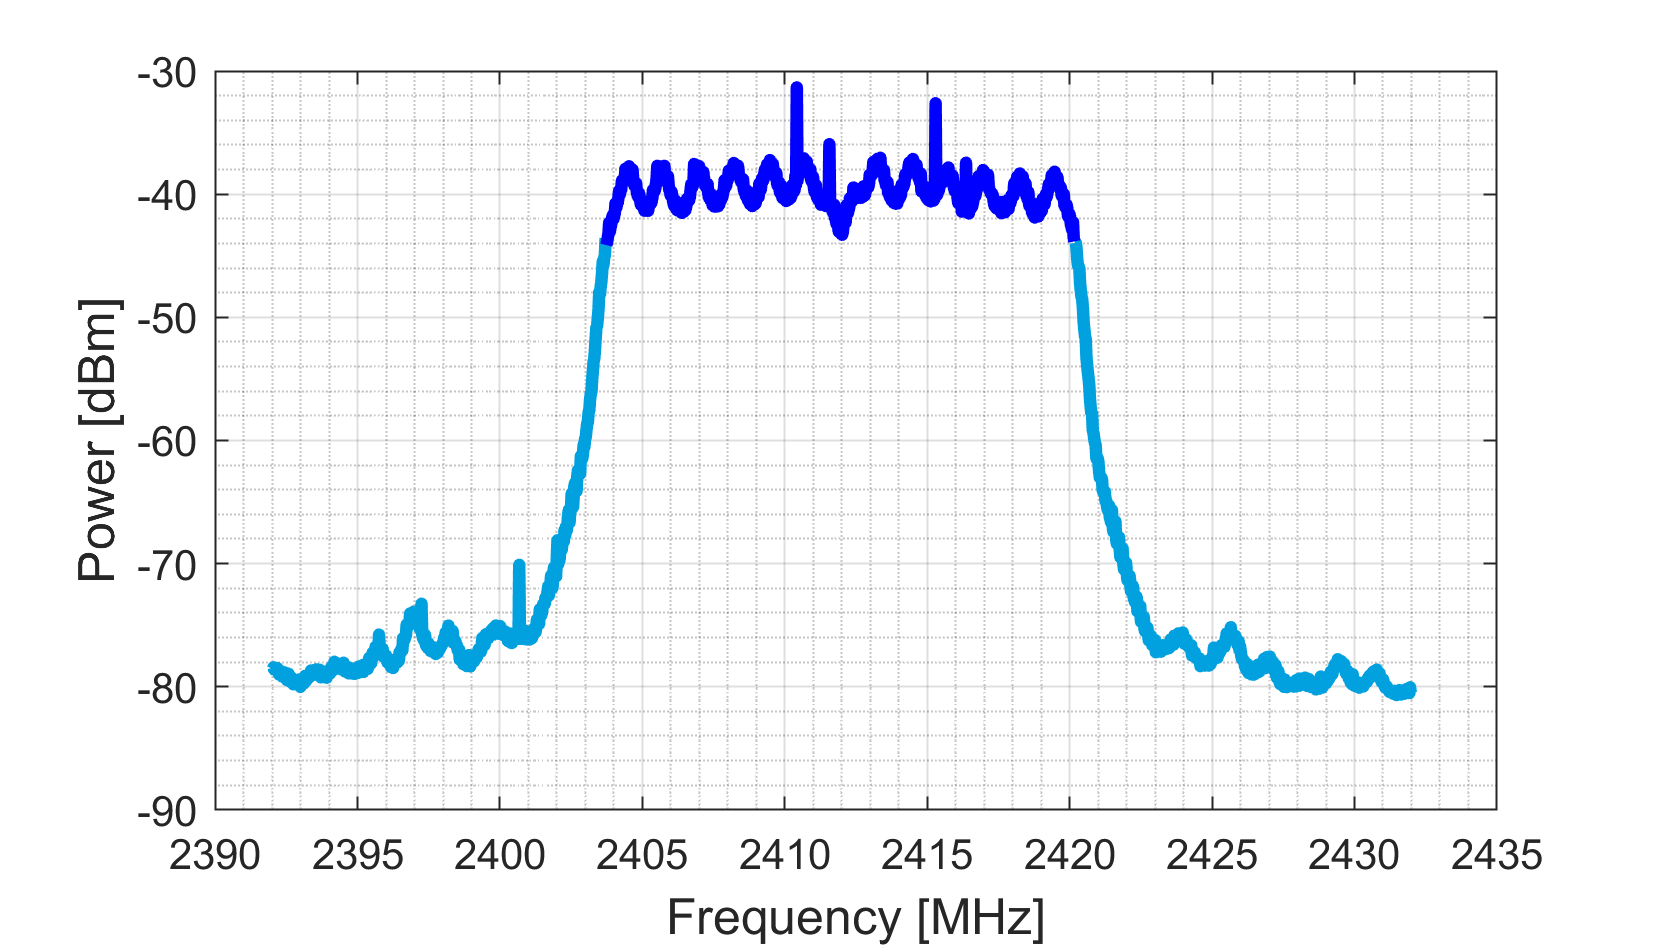
\includegraphics[width=0.65\textwidth]{TraceBandwidth.png}
\caption{Trace of the signal from the analyzer after post processing. The \acs{OBW} is 99\% (dark blue) of the total bandwidth of the signal}
\label{fig:tracebw}
\end{figure}
To locate the occupied channel bandwidth of the signal from the trace produced by the analyzer, we first convert the power value to a linear scale and find the total power. Since we need 99\% of the power, we go in a loop from both sides of the signal (start and stop frequency) and find the value of the frequency on both sides when the power value is 0.5\% of total power. And the difference between the frequency values gives us the 99\% occupied channel bandwidth.
\end{enumerate}
  
\section{\acl{PSD} measurement}
\label{sec:psdmeas}
The \acl{PSD} is the mean \acf{EIRP} spectral density in a 1 MHz bandwidth during a transmission burst. For equipment using wide band modulations other than \acs{FHSS}, the maximum \acf{PSD} is limited to 10 dBm per MHz. This test, like the occupied channel bandwidth measurement, requires the \acs{DUT} to transmit data so that the analyzer can save the trace for the calculation of \acf{PSD}. The steps for this measurement are as follows:

\begin{enumerate}
  \item Associate the DUT with the companion device. Fritz Box acts as a companion device for this measurement. 
\item Run the batch (.BAT) file on the computer connected to the \acs{DUT}. This file uploads data to the \ac{NAS} which is connected to the USB stick on the companion device so that the power spectral density of the \acs{DUT} signal can be measured. Refer section \ref{sec:golden} for the procedure.
\item Change the settings of the spectrum analyzer. The table \ref{tab:analyzerpsd} below contains important analyzer settings.
\begin{table}[ht]
\begin{center}
\begin {tabular} {|c|c|} 
\toprule
Function & Value \\ 
\midrule 
Start frequency & 2400 MHz \\
Stop Frequency  & 2483.5 MHz\\
\ac{RBW} & 10 KHz \\
\ac{VBW} & 30 KHz\\
Sweep points & 8500 \\
Channel Occupancy Time & 10 ms \\
Sweep time & Time on each sweep point * Sweep Points \\
Trace mode & \acs{Max-Hold} \\
Detector & \ac{RMS}\\
\bottomrule
\end{tabular} 
\caption{Spectrum Analyzer settings for \ac{PSD} measurement}
\label{tab:analyzerpsd}
\end{center}
\end{table}
The standard suggests the number of sweep points to be greater than 8350. If the analyzers are not supporting this number of sweep points then the frequency band may be segmented. The measurement device used supports maximum of 15000 sweep points, but sweep points was set to 8500 in this case. Our aim being to reduce \acl{MU}, the sweep count is increased to 10 rather than using a single sweep. The maximum value of trace is saved with the help of \acs{Max-Hold} trace mode.
  
\item Since the signal from the \acs{DUT} is non-continuous, wait for the trace to stabilize and save the trace data to a mat file.
 
 \item Use the following formula to add up the values of power for all sample points.
  $$ P_{sum} = \sum_{n=1}^{k} P_{sample}(n) $$ where k is the total number of samples and n is the actual sample number
  
 \item  Convert the power values from mW scale to dBm scale and then normalize the individual values for power so that the sum is equal to the RF Output Power (\acs{EIRP}) measured in the big anechoic chamber and finally save the corrected data. The following formulas can be used:
  $$C_{corr} = P_{sum} - P_{EIRP}   $$ 
  $$P_{samplecorr}(n) = P_{sample}(n) - C_corr $$ where n is the actual sample number.
  
  \item Starting from the first sample $P_{samplecorr}(n)$ (lowest frequency), sum up the power (in mW) of the following samples representing 1MHz segment and record the results for power and position (i.e. sample 1 to sample 100). This is the Power Spectral Density (\acs{EIRP}) for the first 1 MHz segment.
  
  \item Shift the starting point of the samples by one sample summed up in step 7 and repeat the procedure in step 8. (i.e. sample 2 to sample 101)
  
  \item Repeat step 8 until the end of the data set and record the Power Spectral Density values for each 1 MHz segments. From all the recorded results, the highest value is the maximum Power Spectral Density of the DUT. This value shall be recorded in the test report.
    \end{enumerate}
  
 \begin{figure}[H]
\centering
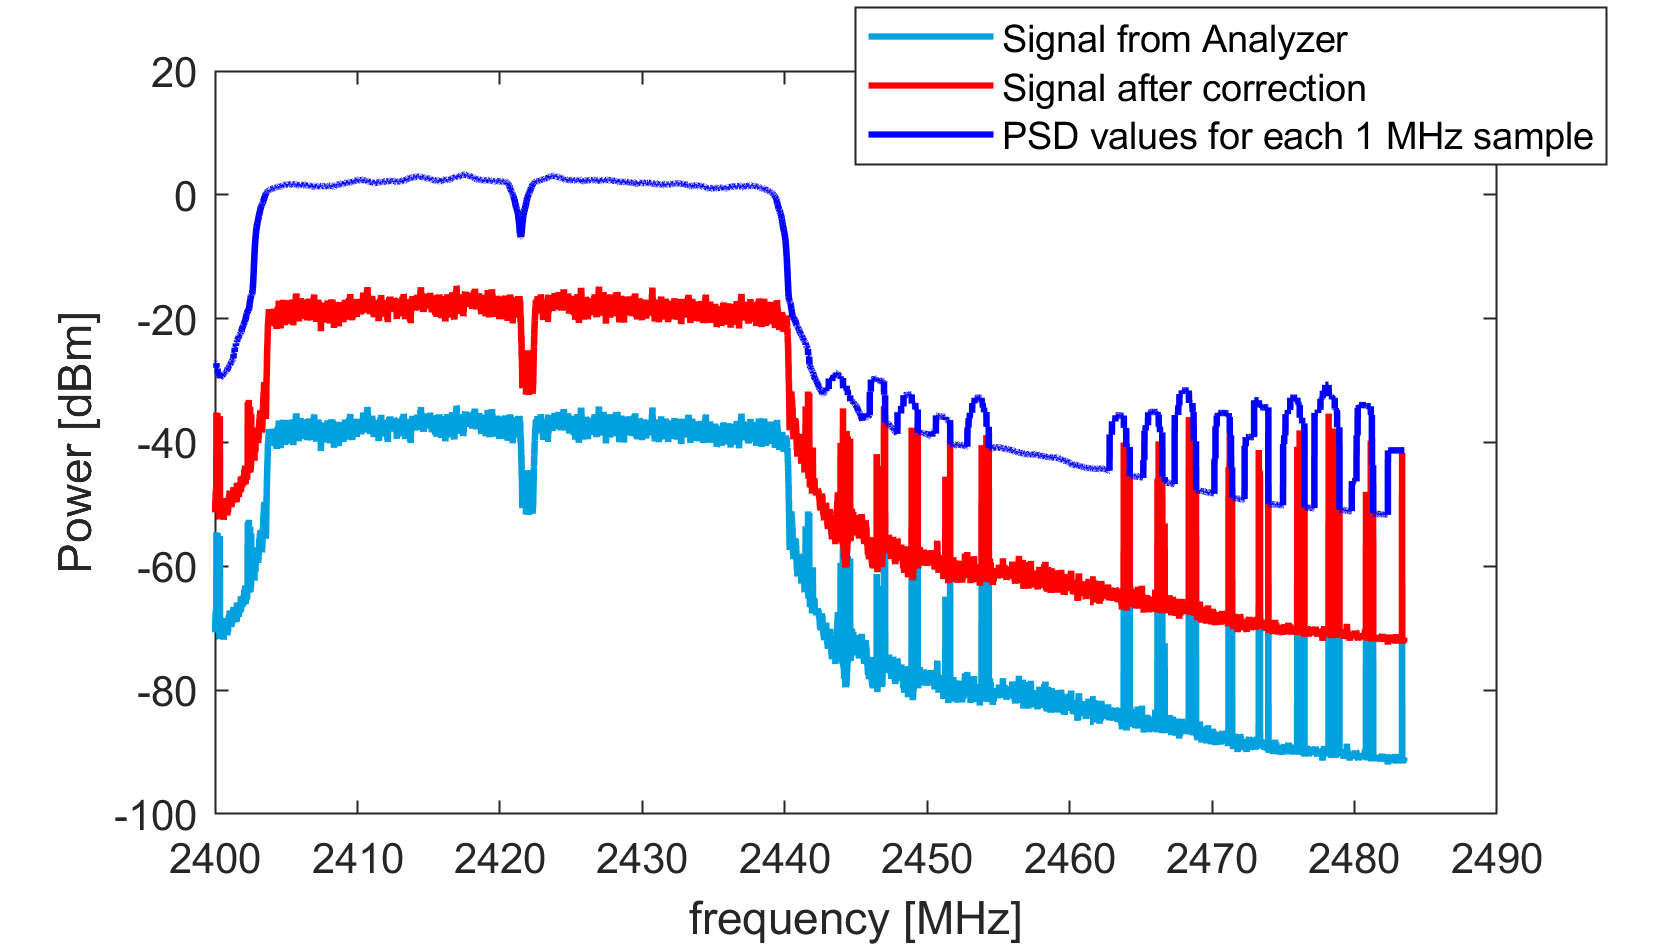
\includegraphics[width=0.75\textwidth]{PSD_trace.png}
\caption{Trace of the signal from the analyzer after post processing. The \acs{PSD} is 3.3015 dBm at 2418 MHz}
\label{fig:psdtraceI}
\end{figure}
  
  
 \section{Receiver Blocking measurement}
\label{sec:rxmeas} 
Receiver blocking is a measure of the ability of the equipment to receive a wanted signal on its operating channel without exceeding a given degradation in the presence of an unwanted signal (blocking signal) at frequencies other than those of the operating band. The minimum performance criterion shall be a \ac{PER} less than or equal to 10 \%. The manufacturer may declare alternative performance criteria as long as that is appropriate for the intended use of the equipment. The procedure for this measurement is explained in the Fig \ref{fig:flowchartrxvlock}.

 \begin{figure}[H]
\centering
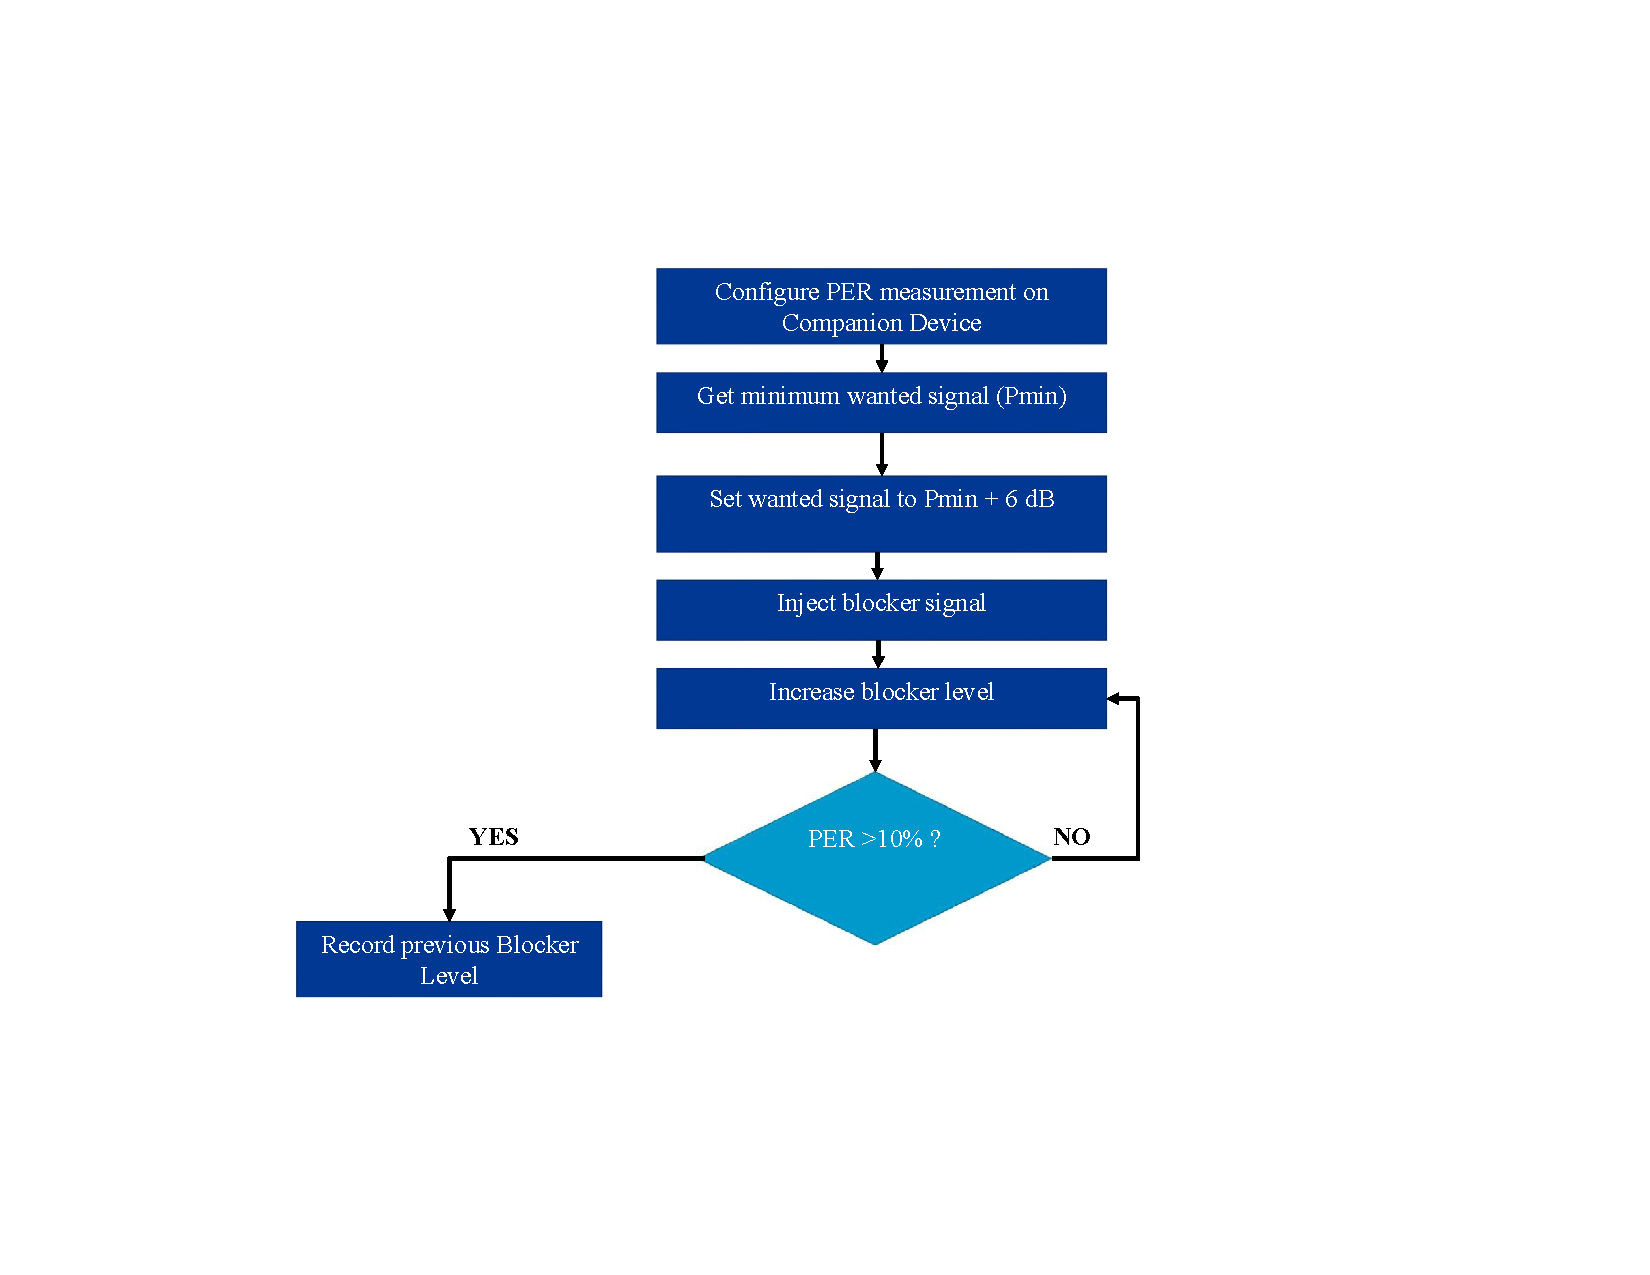
\includegraphics[width=0.9\textwidth]{flowchart.pdf}
\caption{Flowchart for \ac{RxBlocking} measurement}
\label{fig:flowchartrxvlock}
\end{figure}

The association of the \acs{DUT} with the companion is talked about in all other test procedures as well as in the previous chapter. A \acf{PER} measurement is configured on the companion device. The \acs{PER} measurement transmits user data to the \acs{DUT} and calculates the \acs{PER} of acknowledged packets to transmitted packets. The number of MAC test packets to be transmitted is configurable. Each of the test packets carries the same amount of user data to the \acs{DUT}. The test packets can be separated by unused packets. The diagram in the lower part of the dialog shows the \acs{PER} vs time/transmitted packets.

 \begin{figure}[H]
\centering
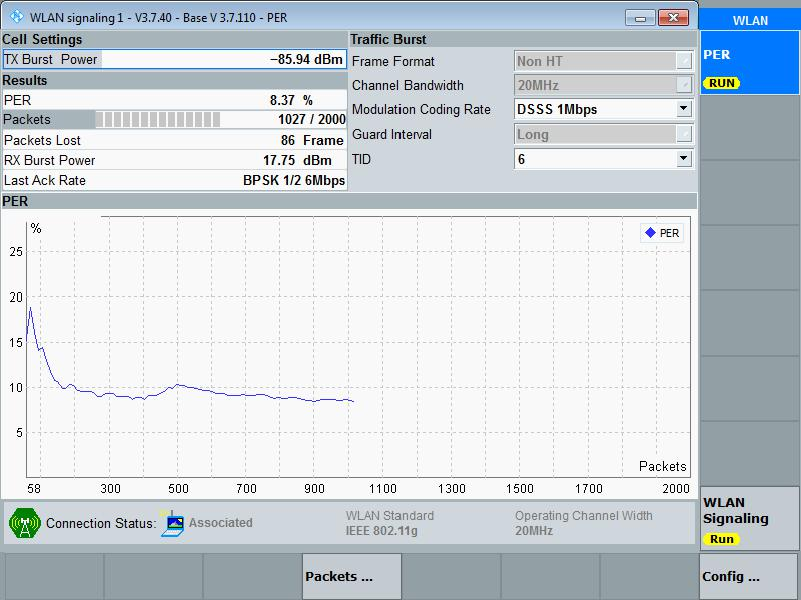
\includegraphics[width=0.75\textwidth]{PER_CMW.jpeg}
\caption{\ac{PER} measurement on the \acs{RS} \acs{CMW}}
\label{fig:per}
\end{figure}

The next phase is to find the minimum wanted signal ($P_{min}$) without the blocker (signal generator). To do this, the power of the transmitted bursts is kept reducing until the \acs{PER} reaches just below 10\%. In order to increase the speed of the measurement, the program first does coarse precision (i.e. reduces power by steps of 1 dBm and sets the transmitted packets to as low as 200). Then for precise measurement, the power is reduced in steps of 0.1 dBm and 2000 packets are transmitted. The \acs{PER} window in the figure above shows the \acs{PER} measurement taking place. \\
  
This is followed by keeping the wanted Signal ($P_{min}$ + 6 dB) constant and injecting a blocker signal using a signal generator at the frequency mentioned in the standard. \acs{PER} measurement then checks for the resulting \acs{PER}. The blocking signal of -34 dBm is applied in front of the \acs{DUT} as mentioned by the standard. Then, the transmitted burst power is kept constant thought-out the measurement by adding 6 dBm to the minimum unwanted signal. The blocker level is kept increasing until the 10\% criterion is reached. This is not required by the standard but it shows us by how much we can take the power level above the value mentioned in the standard. It also gives us an impression of how good the \acs{DUT} performs and allows us to assess the \acf{MU}.




